\section{Ejercicio 2}
\subsection*{Instrucción}
En este apartado se desea implementar la siguiente operación:
\par
\vspace{0.15cm}
\texttt{takeOutOfService(backToService : date):} 
pone un coche que está en servicio fuera de servicio, registra la fecha hasta la que el coche permanecerá fuera de servicio y busca un coche para sustituir al que se pone fuera de servicio. El sustito debe cumplir
una serie de restricciones: 

\begin{itemize}
    \item Debe estar asignado a la misma oficina que el coche sustituido.
    \item Debe ser del mismo modelo.
    \item Finalmente, debe estar en servicio.
\end{itemize}

Además, se menciona la funcionalidad que pone un coche fuera de servicio en servicio. Sin embargo, no se pide su implementación


\subsection{Patrón de Diseño utilizado}

Para poner un coche fuera de servicio hay que considerar varios factores.

Por un lado, el coche que está fuera de servicio no puede ser puesto fuera 
de servicio de nuevo. 

Por otro lado, si un coche está en servicio, pero es sustituto del otro coche, 
tampoco puede ponerse fuera de servicio.

Un coche que está en servicio, puede ser alquilado, mientras que el coche que está fuera de servicio 
o que es el sustituto del otro coche, tampoco puede ser alquilado.

Como se puede apreciar, el comportamiento del coche varía en función de su estado. Por eso, hemos considerado usar el \texttt{Patrón Estados}dado que nos permite definir el comportamient del coche de manera flexible sin cambiar la estructura interna de la clase.

En nuestro caso, un coche puede estar en uno de los dos posibles estados:

\begin{itemize}
    \item \texttt{En servicio:} el coche en este estado está disponible para ser alquilado. 
    \item \texttt{Fuera de servicio:} el coche en este estado está fuera de servicio por varias razones (reparación, ITV, etc.).
    
\end{itemize}



\subsection{Efectos sobre el Diagrama de Diseño}
\begin{figure}[H]
    \centering
     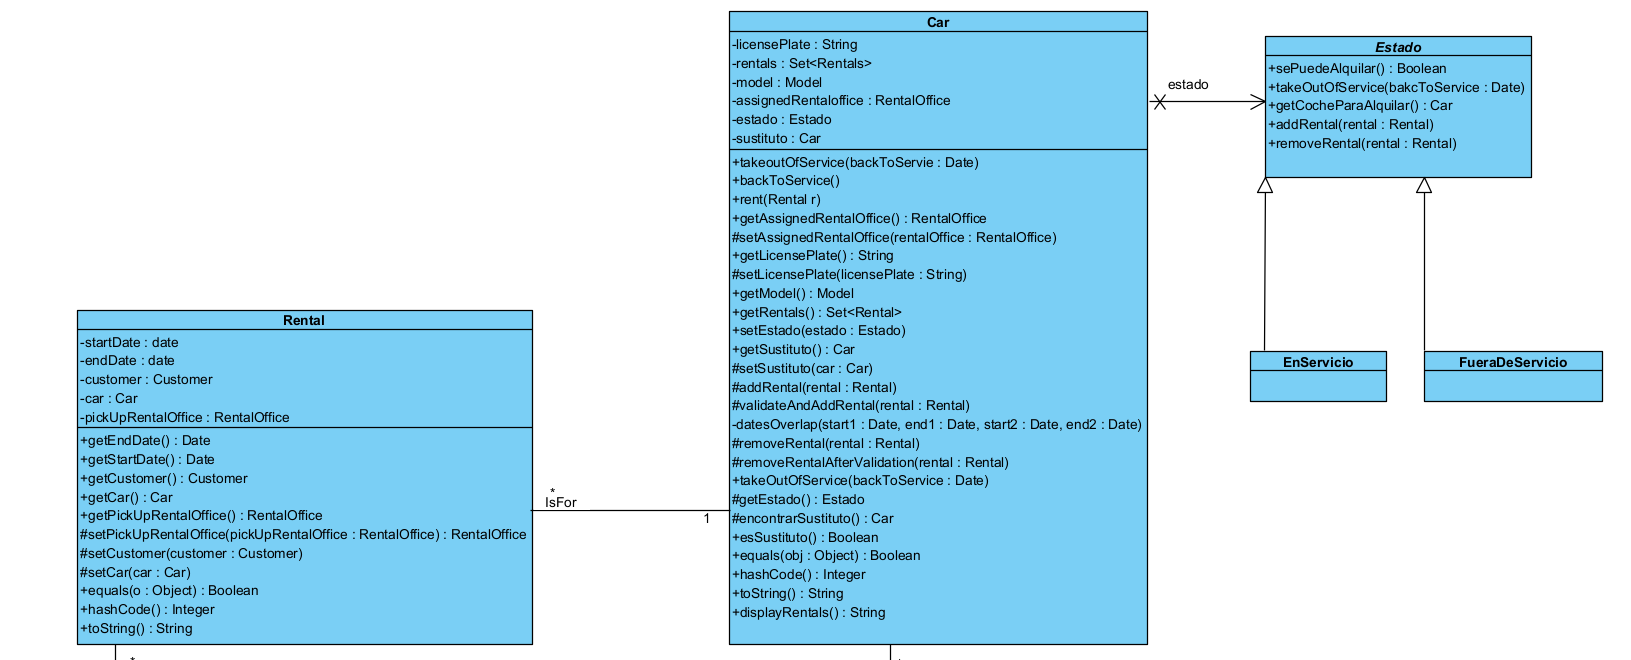
\includegraphics[width=1.0\linewidth]{assets/diagramas/UML_Apartado2.png}
     \caption{Diagrama de Diseño modificado para Ejercicio2}
\end{figure}

Con el fin de implementar el patrón escogido hemos tenido que insertar una clase abstracta \texttt{Estado}
que representa el estado de coche.
Además, hemos tenido que insertar dos clases que heredan de la clase mencionada: 
\begin{itemize}
    \item \texttt{EnServicio:} la instancia de la clase Car con estado de este tipo está en servicio. Este tipo permite poner un
                            coche fuera de servicio y alquilarlo
    \item \texttt{FueraDeServicio:} la instancia de la clase Car con estado de este tipo está fuera de servicio. No permite alquilar un coche, pero permite
                            alquilar el sustituto asociado, si es que existe.
    
\end{itemize}

\subsection*{Métodos adicionales de la calse \texttt{Car}:}
\begin{itemize}
    \item \texttt{protected void validateAndAddRental(Rental rental):} es un método de la calse \texttt{Car} que antes de asignar un alquiler comprueba si 
    no se solapa on ningún otro que ya está asignado al coche. Para realizar esta comprobación se usa un método privado  \texttt{datesOverlap} 

    \begin{lstlisting}[style = javaNormal, language=Java]
      protected void validateAndAddRental(Rental rental) { //Metodo que solo llama el estado, por lo que estamos delegandole la decision
        assert rental != null : "Rental no puede ser null";
        assert !esSustituto() : "El coche esta siendo usado como sustituto";
        for (Rental existingRental : rentals) {
            assert !datesOverlap(existingRental.getStartDate(), existingRental.getEndDate(),
                rental.getStartDate(), rental.getEndDate()) : "El alquiler se solapa con otro ya existente.";
        }
        rentals.add(rental);
    }
   
    \end{lstlisting}
    \item \texttt{protected Car encontrarSustituto():} una vez que el coche se pone fuera de servicio, se usa este método para encontrar sustituto en función de los 
    p usa en la redefinición del método \texttt{takeOutOfService(Date backToService)} en la
    subclase \texttt{EnServicio}, esta parte se trata más adelante. 
    \begin{lstlisting}[style = javaNormal, language=Java]
      protected Car encontrarSustituto(){
        return assignedRentalOffice.getCars().stream()
                .filter(car -> car.getModel().equals(this.getModel()) && car.getEstado().sePuedeAlquilar() && !car.esSustituto())
                .findFirst().orElse(null);

      }
    \end{lstlisting}
    \item \texttt{public boolean esSustituto():} comprueba si el coche actual es sustituto o no. Esta información es necesaria a la hora de 
    asignar un alquiler, dado que si un coche se usa como sustituto no puede ser alquilado como un coche normal.   
    \begin{lstlisting}[style = javaNormal, language=Java]
      public boolean esSustituto(){
        Iterator<Car> iter = this.getModel().getCars().iterator();
        while(iter.hasNext()){
            Car curr = iter.next();
            if(curr.getSustituto() != null && curr.getSustituto().equals(this))
                return true;
        }
        return false;
    }
    \end{lstlisting}
    
\end{itemize}
\subsection*{Métodos de la clase \texttt{Estado}:}
\begin{itemize}
    \item \texttt{public abstract boolean sePuedeAlquilar():} indica si se puede alquilar un coche o si no se puede alquilar un coche. Su implementación en la clase \texttt{EnServicio} 
    devuelve \texttt{verdadero}, mientras que la de la clase \texttt{FueraDeServicio} devuelve \texttt{falso}. Cabe destacar su implementación en la clase \texttt{EnServicio}.
    \begin{lstlisting}[style = javaNormal, language=Java]
        public boolean sePuedeAlquilar(){
          return !context.esSustituto();
        }    
    \end{lstlisting}
    Como se puede observar, usamos el método \texttt{esSustituto()}. Esta implementación, la consideramos correcta dado, que la única condición para 
    que un coche en servicio no se pueda alquilar es que sea un sustituto.
    \begin{lstlisting}[style = javaNormal, language=Java]
        public boolean sePuedeAlquilar(){  return false;}  
    \end{lstlisting}    
    En la clase \texttt{FueraDeServicio} únicamente se devuelve \texttt{false} porque el hecho de que un coche ya esté fuera de servicio es suficiente para que no se pueda alquilar.
    
    \item \texttt{public Car getCocheParaAlquilar():} es un método que devuelve la instancia del coche o el sustituto en función 
    del estado del coche. Al igual que los otros métodos, este tiene dos verisones: una para la clase \texttt{EnServicio}, otra para la clase \texttt{FueraDeServicio}. Empezamos con la primera:
    \begin{lstlisting}[style = javaNormal, language=Java]
        public Car getCocheParaAlquilar() {
           return context; // Devuelve el coche original porque esta en servicio
         }
    \end{lstlisting} 
    Si un coche está en servicio entonces se devuelve la instancia actual.
    \begin{lstlisting}[style = javaNormal, language=Java]
        public Car getCocheParaAlquilar() {
        if (context.getSustituto() != null) {
            return context.getSustituto(); // Devuelve el sustituto si existe
        }
        throw new IllegalStateException("El coche esta fuera de servicio y no tiene sustituto");
        // Devuelve el coche original porque esta en servicio
    }
    \end{lstlisting} 
    Sin embargo, si un coche está fuera de servicio entonces se comprueba si tiene sustituto. En el caso afirmativo, se devuelve el sustituto. En el caso contrario, se lanza una excepción con el mensaje correspondiente. 
    \item \texttt{public boolean addRental(Rental rental):} añade alquiler al propio coche si este está en servicio o al sustituto, si está fuera
    de servicio y tiene uno.

    Si un coche \textbf{está en servicio}, entonces añadimos el nuevo alquiler verificando que es no se solapa con ninguno de los otros asociados al coche. 
  
  \begin{lstlisting}[style = javaNormal, language=Java]
        public void addRental(Rental rental) {
      context.validateAndAddRental(rental);
   }
   // Metodo de la clase Car
   protected void validateAndAddRental(Rental rental) { //Metodo que solo llama el estado, por lo que estamos delegandole la decision
        assert rental != null : "Rental no puede ser null";
        assert !esSustituto() : "El coche esta siendo usado como sustituto";
        for (Rental existingRental : rentals) {
            assert !datesOverlap(existingRental.getStartDate(), existingRental.getEndDate(),
                rental.getStartDate(), rental.getEndDate()) : "El alquiler se solapa con otro ya existente.";
        }
        rentals.add(rental);
    }
   
    \end{lstlisting} 

      Si estuviera \textbf{fuera de servicio}, entonces añadimos el nuevo alquiler al sustituto, si existe, o lanzamos una excepción.
      
    \begin{lstlisting}[style = javaNormal, language=Java]
         public void addRental(Rental rental) {
        if (this.context.getSustituto() != null) {
            context.getSustituto().addRental(rental);
        } else {
            throw new IllegalStateException("El coche esta fuera de servicio y no tiene sustituto");
        }
    }   
    \end{lstlisting}    
    \item \texttt{public boolean removeRental(Rental rental):} sigue la misma lógica que el método \texttt{addRental(Rental rental)}, pero en vez de añadir
    el alquiler, este se elimina.

    Si el coche está en servicio entonces se elimina el alquiler.
    \begin{lstlisting}[style = javaNormal, language=Java]
          public void removeRental(Rental rental) {
      context.removeRentalAfterValidation(rental);
   }
    \end{lstlisting}

    Sin embargo, si el coche está fuera de servicio entonces, o bien se elimina el alquiler del sustituto o se lanza un error si no existe.
    \begin{lstlisting}[style = javaNormal, language=Java]
       public void removeRental(Rental rental) {
        if (this.context.getSustituto() != null){
            context.getSustituto().removeRental(rental);
        }else{
            throw new IllegalStateException("El coche esta fuera de servicio y no tiene sustituto");
        }
    }
    \end{lstlisting}
    
    
\end{itemize}


\subsection{Implementación de \textit{takeOutOfService : date}}

Hemos decidido delegar el método \texttt{takeOutOfService(Date backToService)}  a las subclases de la clase Estado dado que el resultado de la operación depende del estado actual del coche
\vspace{0.5cm}

\begin{lstlisting}[style = javaNormal, language=Java] 

    introducir codigo aqui

\end{lstlisting} % Código en el documento "codigosEj2"
\vspace{0.5cm}
En la clase \texttt{Car} lo único que se hace es delegar la operación de poner el coche fuera del servicio al estado actual de la instancia.\vspace{0.2cm} Si el coche está en servicio, lo primero que tenemos que hacer es comprobar que no es sustituto de ningún otro coche. Si lo es, no se puede poner fuera de servicio.\vspace{0.2cm} Si el coche no es sustituto, se pone fuera de servicio y se busca un sustituto.\vspace{0.2cm}Si el coche ya está fuera de servicio, entonces se lanza una excepción del tipo \texttt{IllegalStateException ()}, indicando que no se puede poner fuera de servicio un coche que ya está fuera de servicio 

\subsection{Testing}
\begin{lstlisting}[style = javaNormal, language=Java]
    import java.text.ParseException;
import java.text.SimpleDateFormat;
import java.util.*;

public class TestA2 {
    public static void main(String[] args) throws ParseException {
        // Crear modelos de coches
        Model modelA = new Model("Model A", 50);

        // Crear oficinas de alquiler
        RentalOffice office1 = new RentalOffice("Office 1", 20);

        // Crear coches
        Car car1 = new Car("ABC-123", modelA, office1);
        Car car2 = new Car("DGJ-324", modelA, office1);
        Car car3 = new Car("XYZ-789", modelA, office1);


       // Ponemos car1 fuera de Servicio:
        SimpleDateFormat sdf = new SimpleDateFormat("yyyy-MM-dd HH:mm:ss");
        Date fecha1 = sdf.parse("2025-01-01 12:00:00");


        //Ponemos car1 fuera de servicio otra vez. No deberia permitirlo

        car1.takeOutOfService(fecha1); // El coche estara fuera de servicio hasta 1 de enero del 2025 y se le asocia el car2

        //Ponemos el car1 fuera de servicio otra vez. Esta vez no lo permite
        //car1.takeOutOfService(fecha1);

        //Ponemos el car2 fuera de servicio. No deberia permitirlo, dado que car2 es sustituto de car1

        //car2.takeOutOfService(fecha1); // El coche estara fuera de servicio hasta 1 de enero del 2025

        //Ponemos car3 fuera de servicio: No deberia de tener un sustituto

        car3.takeOutOfService(sdf.parse("2025-01-12 12:00:00"));

        //Intentamos alquilar un coche que esta fuera de servicio, pero que tiene un sustituto

        Customer c1 = new Customer("12345H", "Fulanito");

        Date startDate = sdf.parse("2024-01-14 12:00:00");
        Date endDate = sdf.parse("2024-01-21 12:00:00");

        Rental rent1 = new RentalOnSite(startDate, endDate, c1, car1, office1); // No funciona bien

        Date startDate2 = sdf.parse("2024-01-14 12:30:00");
        Date endDate2 = sdf.parse("2024-01-21 12:30:00");

        //Ahora vamos a intentar alquilar el coche 2 que esta siendo sustituto del coche 1

        //Descomentar esta linea para comprobar el alquiler de un coche sustituto
        //Rental rent2 = new RentalOnSite(startDate2, endDate2, c1, car2, office1);




        // Intentamos alquilar un coche que esta fuera de servicio y que not tiene sustituto:

        Date startDate3 = sdf.parse("2024-01-14 12:30:00");
        Date endDate3 = sdf.parse("2024-01-21 12:30:00");
        //Falla por intentar alquilar un coche fuera de servicio
        //Rental rent3 = new RentalOnSite(startDate3, endDate3, c1, car3, office1);

        System.out.println(rent1.toString());



    }
}
\end{lstlisting}
\subsubsection*{Output}
Caso 1: 
\vspace{0.15cm}
Fulanito DGJ-324 ; null
\vspace{0.15cm}
Caso 2:
\vspace{0.15cm}
Exception in thread "main" java.lang.AssertionError: La fecha de inicio no es valida
        at Rental.<init>(Rental.java:20)
        at RentalOnSite.<init>(RentalOnSite.java:12)
        at TestA2.main(TestA2.java:54)
\vspace{0.15cm}
Vemos en este caso un error debido a que estamos intentando solapar fechas.
Caso 3:
\vspace{0.15cm}
Exception in thread "main" java.lang.IllegalStateException: El coche está fuera de servicio y no tiene sustituto
        at FueraDeServicio.getCocheParaAlquilar(FueraDeServicio.java:25)
        at Rental.<init>(Rental.java:23)
        at RentalOnSite.<init>(RentalOnSite.java:12)
        at TestA2.main(TestA2.java:64)
        \vspace{0.15cm}
Vemos que aqui tenemos un error debido a que el coche que estamos intentando asociar se encuentra fuera de servicio.
        \newpage